\begin{figure}[H]
  \centering
  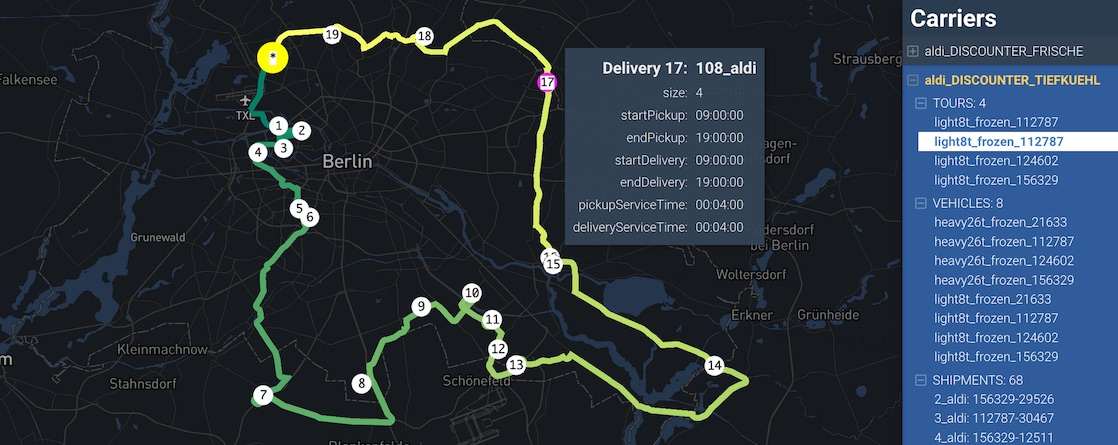
\includegraphics[width=0.8\textwidth]{assets/carriers.jpg}
  \caption{MATSim carrier plans}
\end{figure}


\hypertarget{usage}{%
\subsection{Usage}}

Either the MATSim carriers output file \texttt{output\_carriers.xml}, or a file named \texttt{viz-carrier*.yaml} must be present in the working folder.

If no YAML file is specified and a filename matching pattern "*output\_carriers.xml.gz" is found, it will be loaded with a network file matching the same file pattern.

\textbf{viz-carrier-example.yml}

\begin{lstlisting}
  title: 'Grocery freight network'
  description: '2020 Project'
  network: output_network.xml.gz
  carriers: output_carriers.xml.gz
  center: [13.391, 52.515]
\end{lstlisting}

\hypertarget{yaml-fields-explained}{%
\subsection{YAML fields explained}}

\noindent\textbf{network:} Network filename. Both \texttt{.json.gz} and \texttt{xml.gz} network
files are supported, but JSON-based files load \emph{much} faster.

\noindent\textbf{carriers:} Name of the output\_carriers xml file

\noindent\textbf{center:} Use this to force the map center point.
\texttt{{[}long,lat{]}}
